\documentclass[12pt,a4paper]{article}
\usepackage[utf8]{inputenc}
\usepackage[T1]{fontenc}
\usepackage{lmodern}
\usepackage[french]{babel}
\usepackage{graphicx}
\usepackage{geometry}
\usepackage{float}
\usepackage{caption}
\usepackage{tikz}
\usepackage{tabularx}
\usepackage{booktabs}
\usepackage{array}
\usepackage{enumitem}
\usepackage{amsmath,amsfonts,amssymb}
\usepackage{url}
\usepackage{titlesec}
\usepackage{fancyhdr}
\usepackage{xcolor}
\usepackage{microtype}
\usepackage[colorlinks=true,linkcolor=blue!75!black,citecolor=blue!75!black,urlcolor=blue!75!black]{hyperref}

% --- Configuration de la mise en page ---
\geometry{a4paper, margin=2cm, headheight=15pt, bottom=2.2cm}
\setlength{\parindent}{0pt}
\setlength{\parskip}{0.55em}
\addto\captionsfrench{\renewcommand{\contentsname}{Sommaire}}
\addto\captionsfrench{\renewcommand{\listfigurename}{Table des figures}}
\addto\captionsfrench{\renewcommand{\listtablename}{Liste des tableaux}}

% --- Configuration des légendes et listes ---
\captionsetup[figure]{font=small, labelfont=bf, justification=centering, margin=0.6cm}
\captionsetup[table]{font=small, labelfont=bf, justification=centering, margin=0.6cm}
\setlist[itemize]{leftmargin=*, itemsep=0.25em, topsep=0.25em}
\setlist[enumerate]{leftmargin=*, itemsep=0.25em, topsep=0.25em}

% --- Configuration des en-têtes et pieds de page ---
\pagestyle{fancy}
\fancyhf{}
\fancyhead[L]{\small\textit{Master 2 Automatique \& Robotique --- UCA EUPI}}
\fancyhead[R]{\small\textit{TP Commande d'un axe vertical}}
\fancyfoot[C]{\thepage}
\renewcommand{\headrulewidth}{0.4pt}
\renewcommand{\footrulewidth}{0.4pt}

% --- Configuration des titres ---
\titleformat{\section}{\normalfont\Large\bfseries\color{blue!80!black}}{\thesection}{1em}{}
\titleformat{\subsection}{\normalfont\large\bfseries\color{black!90}}{\thesubsection}{1em}{}
\titleformat{\subsubsection}{\normalfont\normalsize\bfseries\color{black!80}}{\thesubsubsection}{1em}{}
\titleformat{\part}[display]{\centering\normalfont\Huge\bfseries\color{blue!80!black}}{\Large\partname\ \thepart}{0.4em}{}

\begin{document}

% ==============================================================================
% PAGE DE GARDE
% ==============================================================================
\hypersetup{pageanchor=false}
\begin{titlepage}
    \noindent
    \begin{minipage}{0.45\textwidth}
        \begin{flushleft}
            
\includegraphics[width=4.2cm]{img_garde/logo_uca.png}
        \end{flushleft}
    \end{minipage}
    \hfill
    \begin{minipage}{0.45\textwidth}
        \begin{flushright}
            
\includegraphics[width=6.8cm]{img_garde/logo_eupi.png}
        \end{flushright}
    \end{minipage}

    \vspace{1.2cm}

    \begin{center}
        {\Large \textsc{UNIVERSITÉ CLERMONT AUVERGNE}}\\[0.2cm]
        {\large Clermont-Ferrand}\\[0.4cm]

        \rule{0.12\textwidth}{0.6pt}\\[0.4cm]

        {\large École Universitaire de Physique et d'Ingénierie}\\[0.4cm]

        \rule{0.12\textwidth}{0.6pt}\\[1.2cm]

        {\LARGE \textbf{COMPTE RENDU DE TRAVAUX PRATIQUES}}\\[0.4cm]
        {\large 2\textsuperscript{e} année de Master}\\[0.3cm]
        {\large Spécialité : \textbf{Automatique et Robotique}}\\[1.2cm]

        {\large \textbf{Auteurs (Groupe 3) :}}\\[0.2cm]
        {\large \textbf{Romaric PRADEAU}}\\[0.15cm]
        {\large \textbf{Baptiste CHAZAL}}\\[0.15cm]
        {\large \textbf{Beraldo Welcome MOUSSOUNGOU}}\\[1.5cm]

        {\Huge \textbf{Commande d'un Axe Vertical}}\\[0.4cm]
        {\Large \textit{Réglage automatique sous PME, analyse des frottements et identification mécanique}}\\[1.8cm]
    \end{center}

    \vfill

    \begin{flushleft}
        \large
        \textbf{Date :} Octobre 2026\\[0.2cm]
        \textbf{Matière :} Commande des actionneurs électriques \& Asservissements numériques
    \end{flushleft}
\end{titlepage}
\hypersetup{pageanchor=true}

\pagenumbering{roman}

% ==============================================================================
% INTRODUCTION
% ==============================================================================
\section*{Introduction}
\addcontentsline{toc}{section}{Introduction}

La commande précise d'axes électromécaniques verticaux représente une problématique fondamentale en automatique appliquée et en robotique industrielle (transstockeurs, manipulateurs verticaux, ascenseurs de charge, portiques d'usinage). Contrairement aux axes horizontaux, un axe vertical est soumis de façon permanente à l'accélération de la pesanteur. Cette dissymétrie physique introduit un couple gravitationnel constant unidirectionnel qui altère significativement la dynamique du système, en particulier lors des transitions entre montée et descente, ainsi qu'aux très faibles vitesses où les non-linéarités de frottement sec jouent un rôle prépondérant.

Le présent travail pratique a pour support un banc électromécanique composé d'un chariot mobile guidé verticalement, entraîné par un servomoteur synchrone via un réducteur mécanique et une transmission par poulie-courroie crantée. L'étude menée s'articule autour de deux axes complémentaires :
\begin{enumerate}
    \item \textbf{Étude et évaluation du réglage automatique sous le logiciel PME :} analyser l'influence des paramètres clés de l'asservissement numérique --- le gain proportionnel de position ($K_p$), la compensation du moment d'inertie de la charge ($J$), et l'action d'anticipation de consigne (\textit{Feedforward}) --- sur les erreurs de traînage et sur les instabilités à basse vitesse causées par le frottement statique (phénomène de \textit{stick-slip}) ;
    \item \textbf{Mise en œuvre d'une procédure de réglage orienté mécanique par identification expérimentale :} caractériser finement le comportement physique du banc en dissociant et en quantifiant le couple de pesanteur ($C_{\text{grav}}$), la caractéristique complète de frottement (frottement sec de Coulomb $f_s$ et coefficient de frottement visqueux $f$) ainsi que le moment d'inertie global équivalent ($J_{\text{tot}}$) ramené à l'arbre moteur. Cette identification permettra de synthétiser les correcteurs des boucles imbriquées de vitesse et de position selon les gabarits fréquentiels constructeur, puis d'analyser les limites dynamiques de l'actionneur physique en régime de fortes sollicitations.
\end{enumerate}

\clearpage
\pagenumbering{arabic}

% ==============================================================================
% SOMMAIRE
% ==============================================================================
\tableofcontents
\clearpage

% ==============================================================================
% PARTIE I : PROCÉDURE DE RÉGLAGE AUTOMATIQUE SOUS PME
% ==============================================================================
\part{Procédure de réglage automatique sous PME}

\section{Plan expérimental et calcul théorique préliminaire}
\label{sec:plan_exp}

\subsection{Objectifs et matrice des essais}

Afin d'évaluer de manière systématique l'influence de chaque composante de la boucle d'asservissement, cinq expérimentations successives ont été réalisées sur le banc d'axe vertical en faisant varier :
\begin{itemize}
    \item \textbf{Le gain proportionnel ($K_p$) :} règle la raideur de rappel de la boucle de position et sa réactivité face aux écarts de poursuite ;
    \item \textbf{L'inertie déclarée ($J$) :} valeur communiquée au régulateur pour adapter la dynamique de la boucle de vitesse ($J = 0$ pour une charge déclarée nulle, ou $J = J_{\text{charge}}$ pour l'inertie nominale de la charge) ;
    \item \textbf{L'anticipation de consigne (\textit{Feedforward}) :} anticipation en boucle ouverte basée sur la dérivée du profil de trajectoire, injectant instantanément l'effort requis pour suivre la vitesse et l'accélération sans dépendre exclusivement du signal d'erreur de position.
\end{itemize}

Le tableau~\ref{tab:manipulations} détaille la matrice des configurations expérimentales testées au cours de cette première phase.

\begin{table}[H]
\centering
\begin{tabular}{cccc}
\toprule
\textbf{Expérimentation} & \textbf{Gain proportionnel ($K_p$)} & \textbf{Inertie ($J$)} & \textbf{Feedforward} \\
\midrule
Manipulation 1 & $33$  & $0$                     & Off \\
Manipulation 2 & $100$ & $0$                     & Off \\
Manipulation 3 & $100$ & $J_{\text{charge}}$     & Off \\
Manipulation 4 & $100$ & $0$                     & On  \\
Manipulation 5 & $100$ & $J_{\text{charge}}$     & On  \\
\bottomrule
\end{tabular}
\caption{Synthèse des configurations expérimentales testées lors du réglage PME}
\label{tab:manipulations}
\end{table}

\clearpage

\subsection{Calcul théorique de l'inertie de la charge ramenée au moteur}

Préalablement à l'acquisition des mesures, il est nécessaire d'estimer théoriquement le moment d'inertie équivalent de la masse en translation ramené sur l'arbre rotorique du servomoteur, noté $J_{\text{charge}}$. Les caractéristiques cinématiques et massiques du banc sont les suivantes :
\begin{itemize}
    \item Rapport de réduction du réducteur à engrenages : $r = 8$ ;
    \item Rayon primitif de la poulie crantée motrice : $R = 4{,}3\,\text{cm} = 0{,}043\,\text{m}$ ;
    \item Masse totale du chariot mobile à vide : $M = 10{,}5\,\text{kg}$.
\end{itemize}

La puissance cinétique développée par la masse mobile en translation $v(t) = \frac{R}{r}\,\Omega_m(t)$ équivaut à celle d'un solide de moment d'inertie équivalent $J_{\text{charge}}$ en rotation pure à la vitesse de l'arbre moteur $\Omega_m(t)$ :
\begin{equation}
E_c = \frac{1}{2} \, M \, v^2 = \frac{1}{2} \, M \left(\frac{R}{r} \, \Omega_m\right)^2 = \frac{1}{2} \, J_{\text{charge}} \, \Omega_m^2
\end{equation}

On en déduit l'expression analytique du moment d'inertie équivalent ramené au rotor :
\begin{equation}
J_{\text{charge}} = \frac{M \, R^2}{r^2}
\label{eq:formule_inertie}
\end{equation}

L'application numérique donne :
\begin{equation}
J_{\text{charge}} = \frac{10{,}5 \times 0{,}043^2}{8^2} = \frac{10{,}5 \times 0{,}001849}{64} \approx 3{,}03 \times 10^{-4}\,\text{kg}\cdot\text{m}^2
\label{eq:calcul_inertie}
\end{equation}

Cette grandeur sert de paramètre de consigne pour configurer l'inertie de charge dans le progiciel PME ($J_{\text{charge}} \approx 0{,}000303\,\text{kg}\cdot\text{m}^2$).

\clearpage

\section{Analyse des essais expérimentaux}

\subsection{Manipulation 1 : \texorpdfstring{$K_p = 33$}{Kp = 33}, Inertie \texorpdfstring{$= 0$}{= 0}, Feedforward Off}

Cette manipulation initiale correspond à un asservissement volontairement sous-calibré : gain proportionnel modéré, compensation d'inertie nulle et absence d'anticipation. L'ensemble des grandeurs temporelles enregistrées est illustré sur la figure~\ref{fig:manip1_globale}.

\begin{figure}[H]
    \centering
    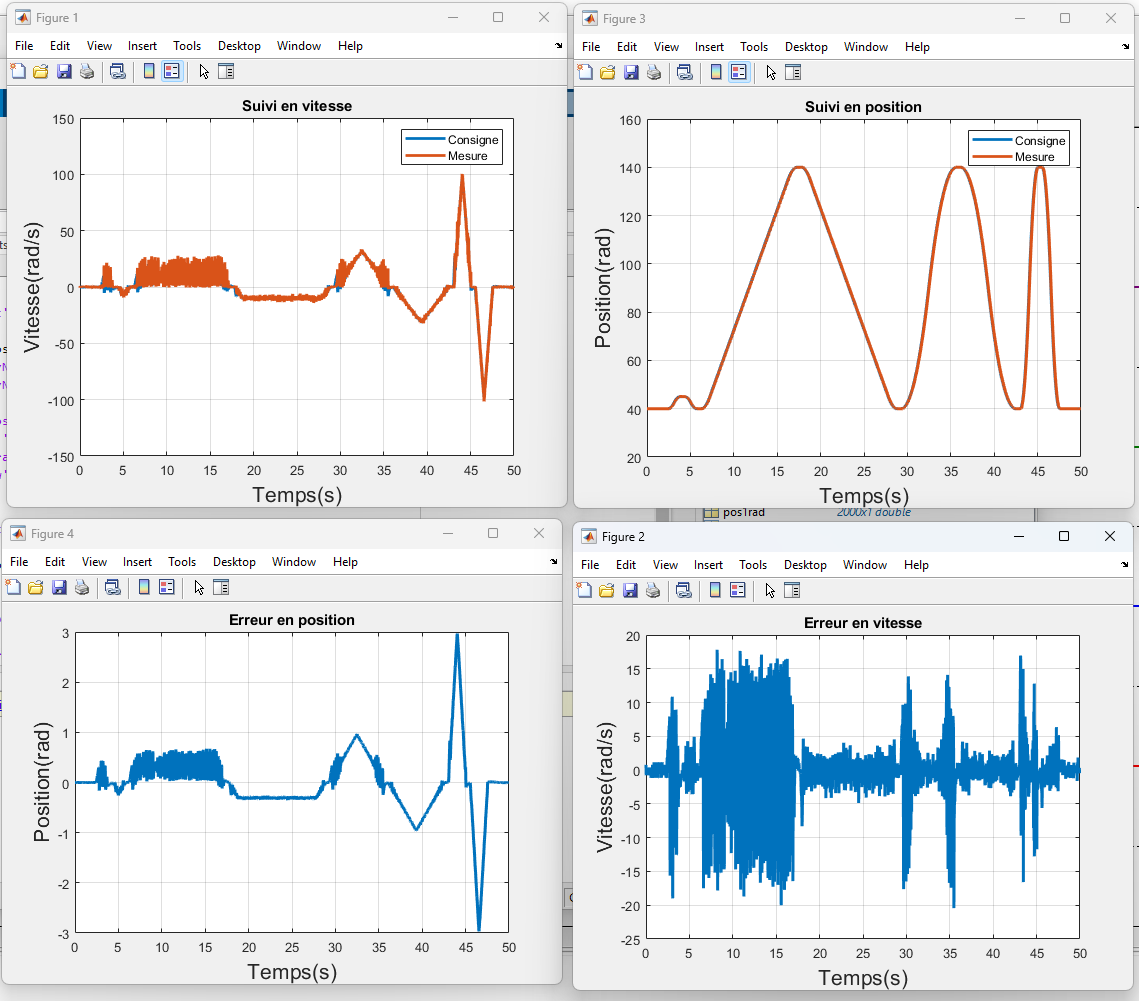
\includegraphics[width=0.72\textwidth]{src/image3.png}
    \caption{Relevés globaux de la Manipulation 1 ($K_p = 33$, $J = 0$, Feedforward Off) : suivi et erreurs en vitesse et position}
    \label{fig:manip1_globale}
\end{figure}

Les courbes globales révèlent une importante erreur de vitesse transitoire (pouvant atteindre $15\,\text{rad/s}$) ainsi qu'un traînage prononcé en position. Une observation détaillée du suivi de position au cours des trois montées consécutives (figures~\ref{fig:manip1_m1}, \ref{fig:manip1_m2} et \ref{fig:manip1_m3}) met en évidence des singularités locales majeures.

\begin{figure}[H]
    \centering
    \begin{minipage}{0.32\textwidth}
        \centering
        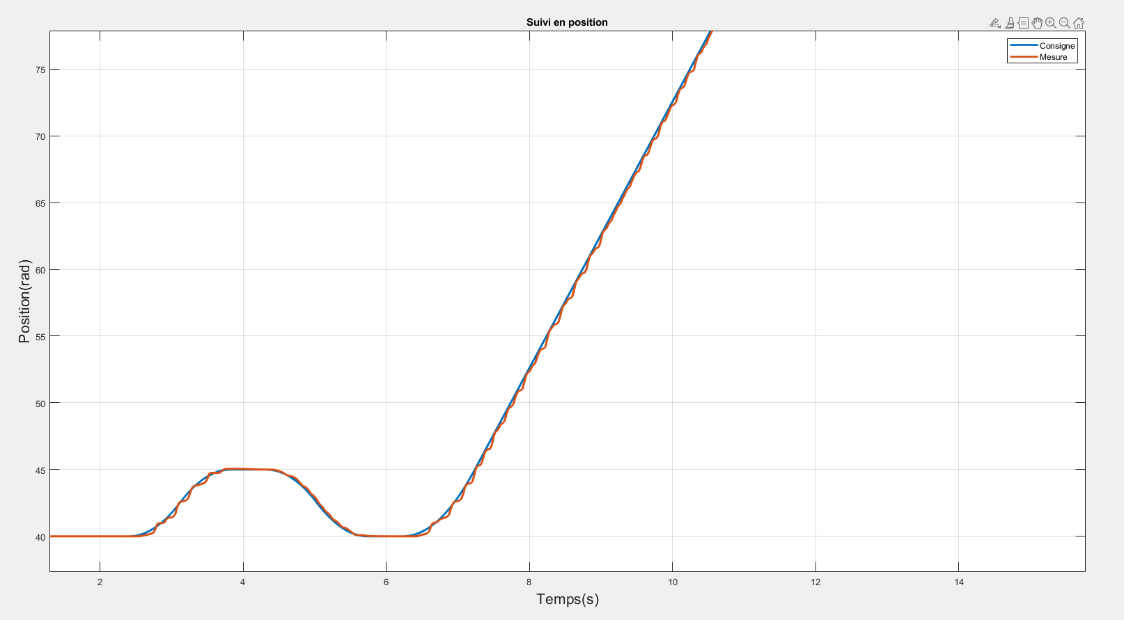
\includegraphics[width=\linewidth]{src/image4.png}
        \caption{1\textsuperscript{re} montée}
        \label{fig:manip1_m1}
    \end{minipage}
    \hfill
    \begin{minipage}{0.32\textwidth}
        \centering
        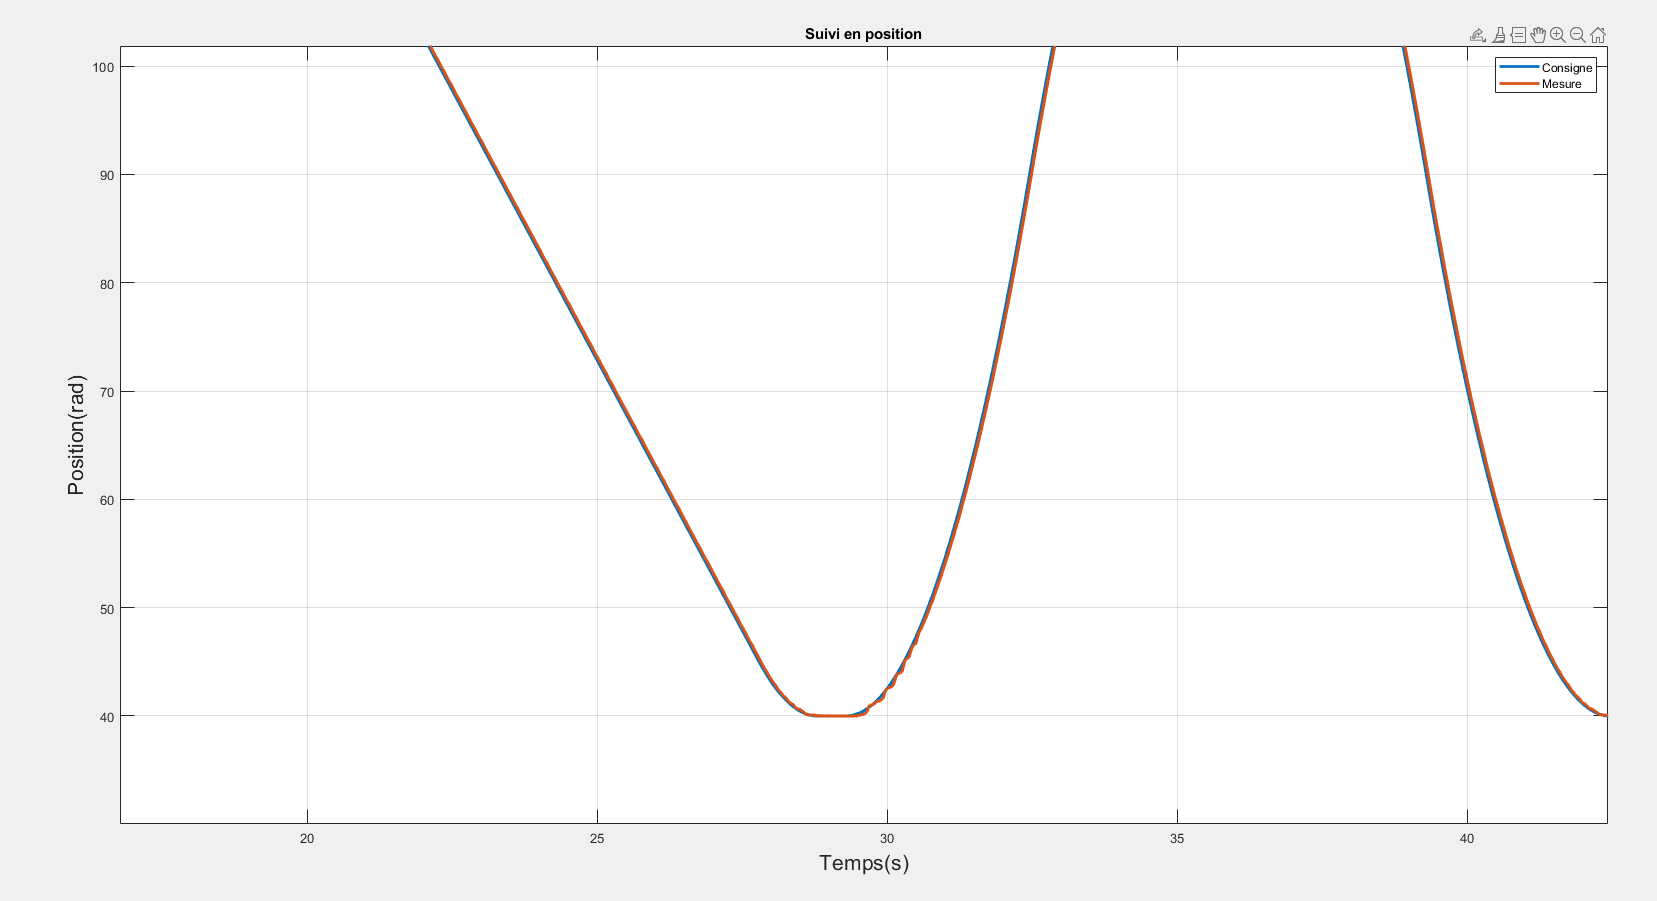
\includegraphics[width=\linewidth]{src/image5.png}
        \caption{2\textsuperscript{e} montée}
        \label{fig:manip1_m2}
    \end{minipage}
    \hfill
    \begin{minipage}{0.32\textwidth}
        \centering
        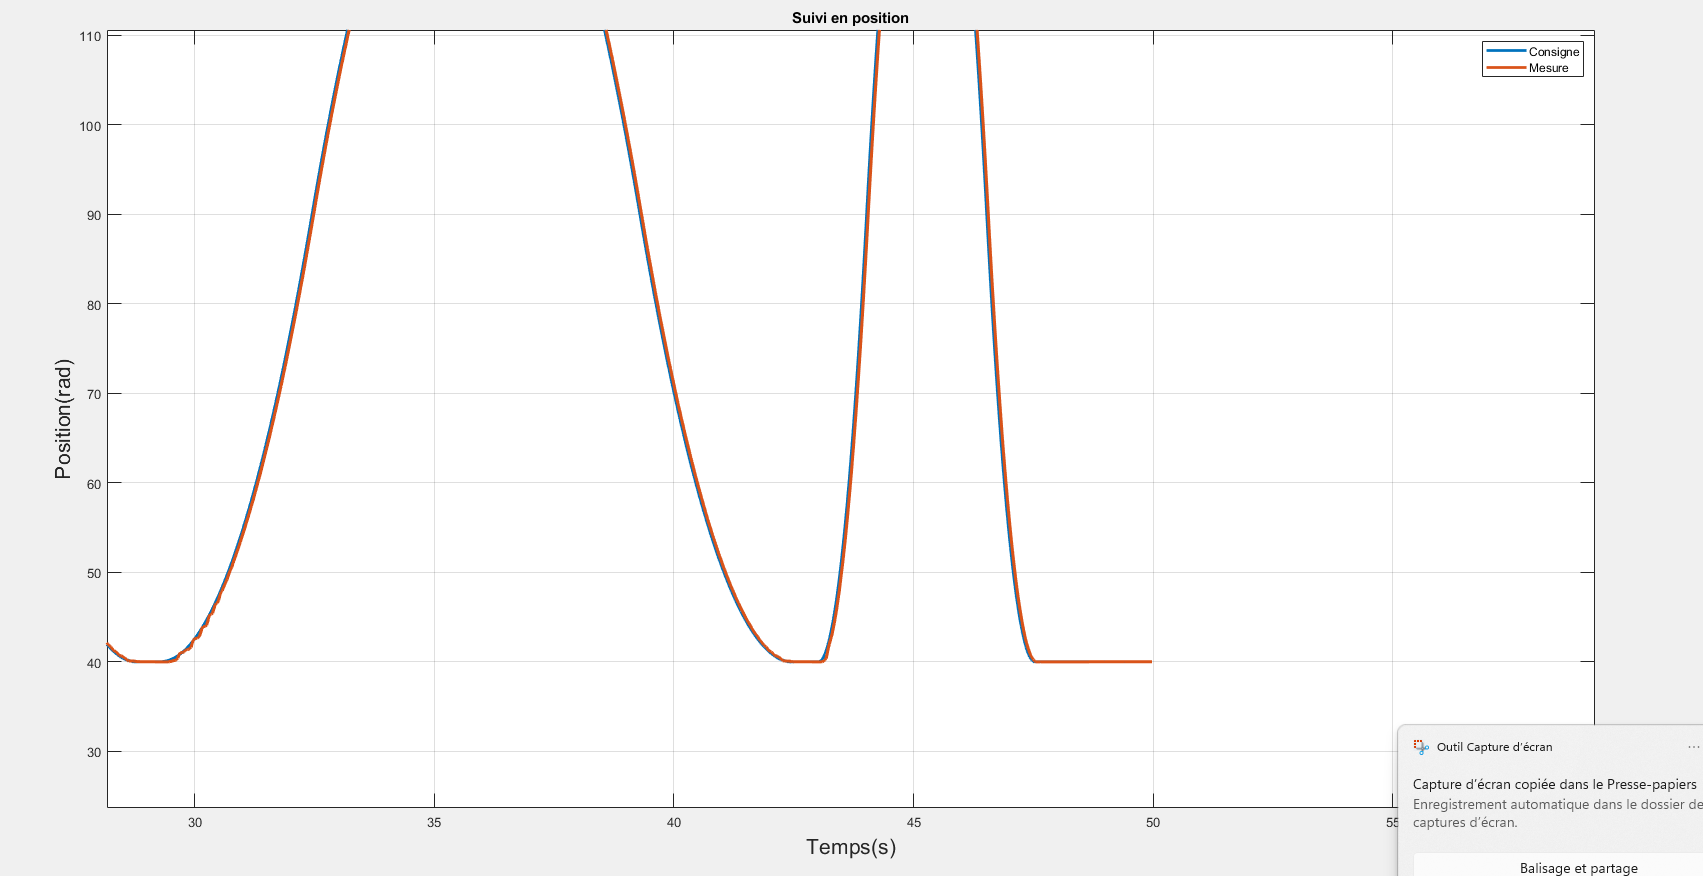
\includegraphics[width=\linewidth]{src/image6.png}
        \caption{3\textsuperscript{e} montée}
        \label{fig:manip1_m3}
    \end{minipage}
    \caption{Agrandissement du suivi de position lors des trois montées consécutives (Manipulation 1)}
    \label{fig:manip1_zooms}
\end{figure}

\textbf{Interprétation physique des résultats :}
\begin{enumerate}
    \item \textbf{Phénomène de saccade et d'adhérence (\textit{stick-slip}) :} Sur la première montée (figure~\ref{fig:manip1_m1}), la réponse mesurée se décompose en paliers discrets formant des « marches d'escalier », particulièrement marqués au décollage et à l'approche de la consigne stabilisée. À ces faibles vitesses, le frottement statique (adhérence) domine. Avec un gain faible $K_p = 33$, l'erreur de poursuite engendre un couple moteur insuffisant pour décoller la charge ; l'axe demeure bloqué (\textit{stick}). Lorsque l'écart de position cumulé produit un couple supérieur au seuil critique de frottement sec, l'axe décroche brusquement en accélération (\textit{slip}), rattrape la consigne, puis se bloque de nouveau dès que la vitesse s'annule.
    \item \textbf{Dissymétrie montée/descente :} Ce phénomène d'escalier est absent en phase de descente. La pesanteur agit alors comme une force motrice auxiliaire orientée dans le sens de la consigne, ce qui aide le système à franchir spontanément la barrière d'adhérence statique.
    \item \textbf{Atténuation temporelle :} L'effet d'escalier tend à s'estomper entre la première et la troisième montée (figures~\ref{fig:manip1_m2} et \ref{fig:manip1_m3}). Ce comportement résulte de l'échauffement progressif des surfaces de contact mécanique et d'une meilleure répartition du film de graisse sur les rails de guidage, abaissant le coefficient de frottement statique effectif.
\end{enumerate}

\subsection{Manipulation 2 : \texorpdfstring{$K_p = 100$}{Kp = 100}, Inertie \texorpdfstring{$= 0$}{= 0}, Feedforward Off}

Dans le but d'augmenter la raideur dynamique de l'asservissement, le gain proportionnel de position est accru à $K_p = 100$, tout en maintenant l'inertie à zéro et l'anticipation désactivée.

\begin{figure}[H]
    \centering
    \begin{minipage}{0.55\textwidth}
        \centering
        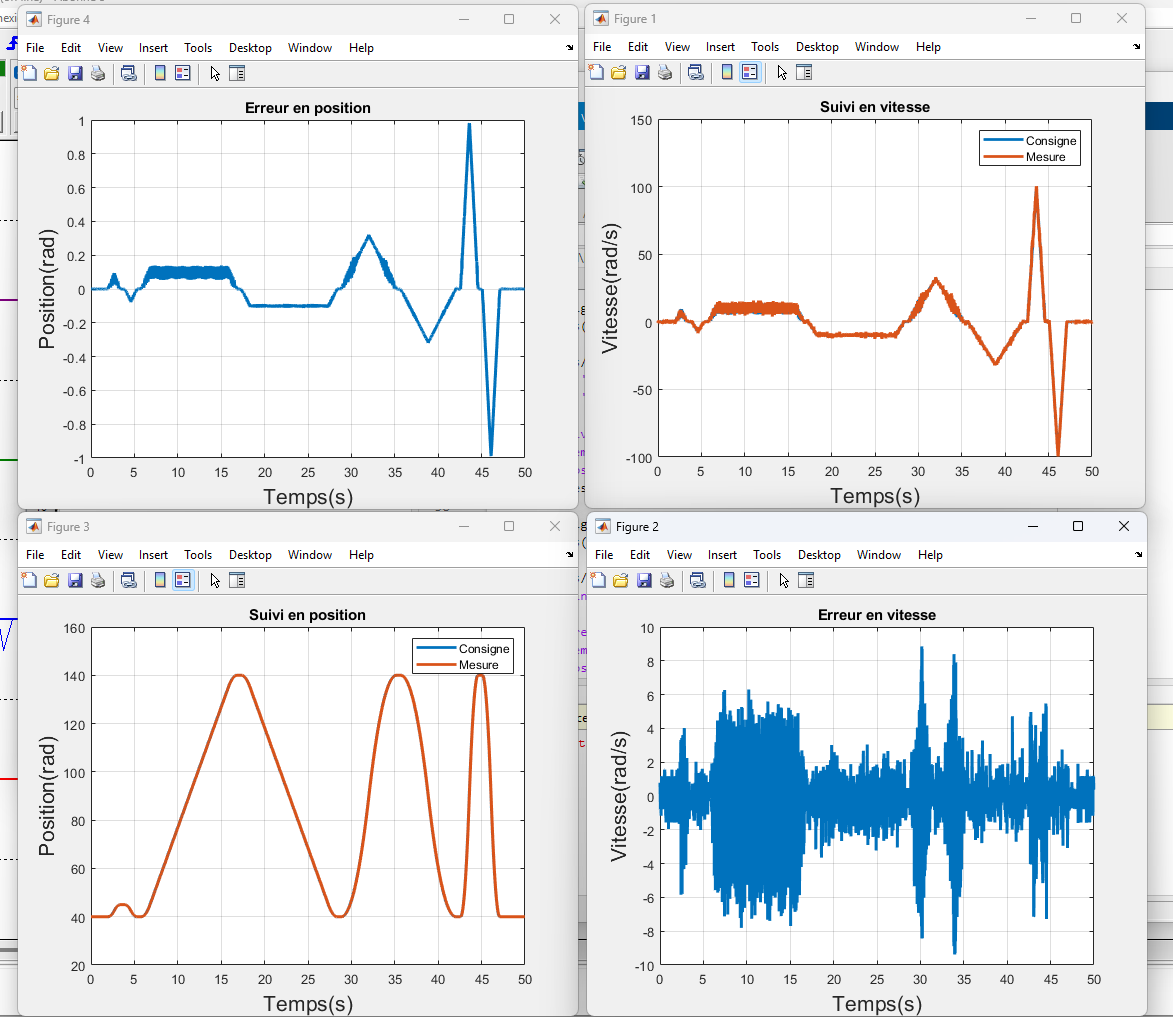
\includegraphics[width=\linewidth]{src/image7.png}
        \caption{Relevé temporel global (Manipulation 2)}
        \label{fig:manip2_globale}
    \end{minipage}
    \hfill
    \begin{minipage}{0.41\textwidth}
        \centering
        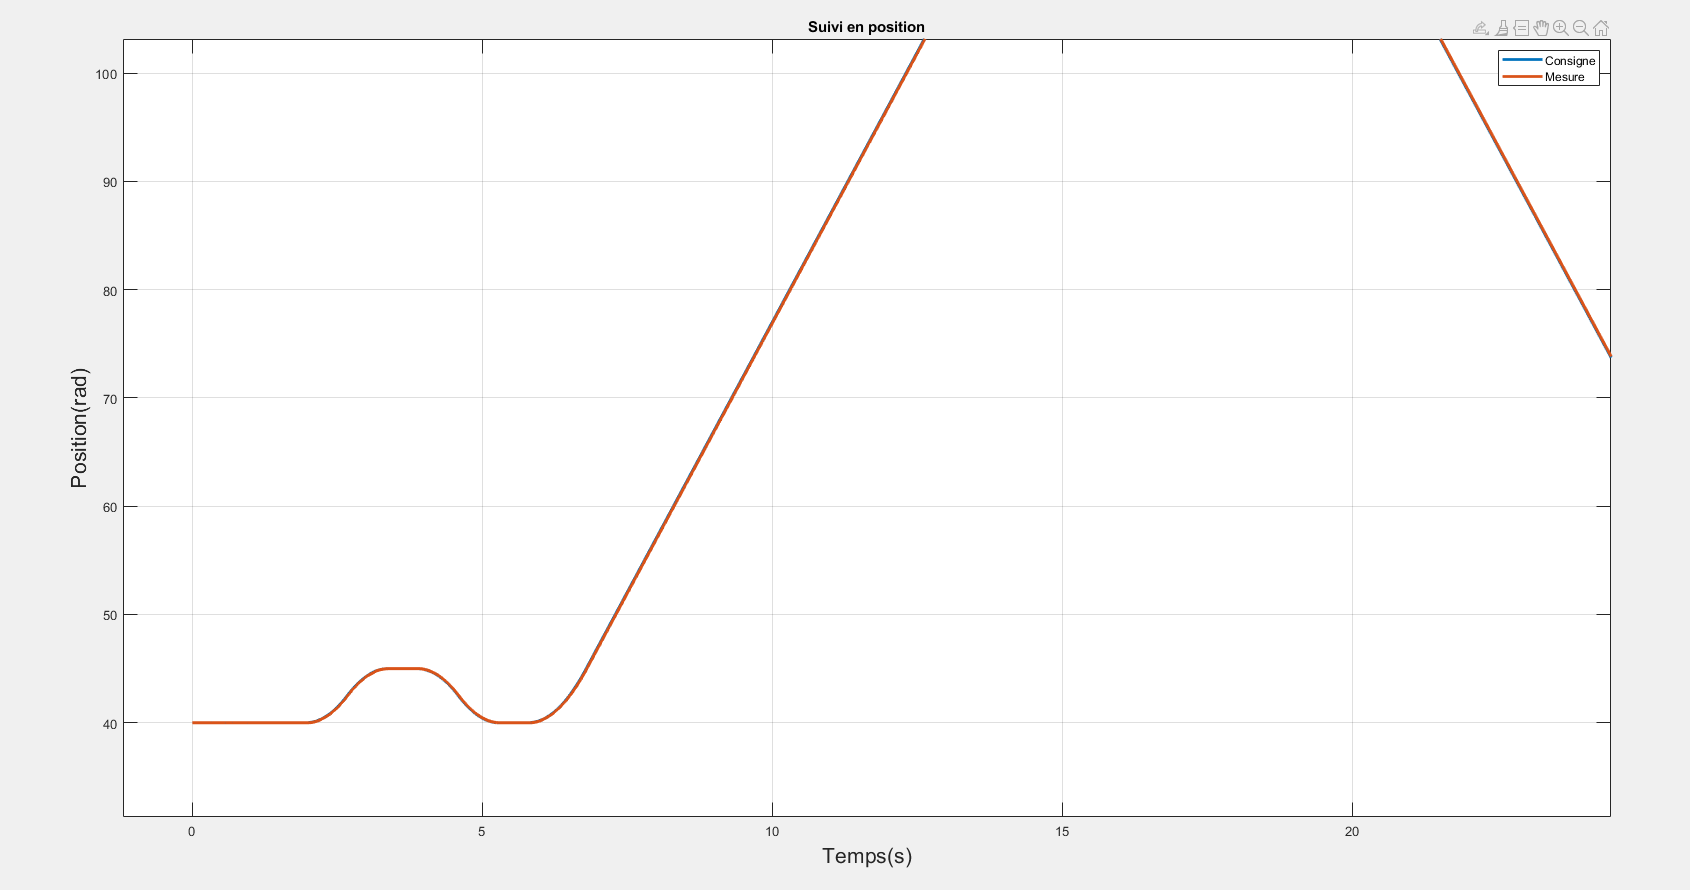
\includegraphics[width=\linewidth]{src/image8.png}
        \caption{Zoom sur le suivi de position}
        \label{fig:manip2_zoom}
    \end{minipage}
\end{figure}

\textbf{Résultats et analyse comparative :}
L'augmentation du gain proportionnel apporte deux améliorations déterminantes :
\begin{itemize}
    \item \textbf{Atténuation des erreurs de poursuite :} L'erreur dynamique en vitesse est divisée par trois lors des phases d'accélération (figure~\ref{fig:manip2_globale}), garantissant une conformité accrue avec la rampe de consigne.
    \item \textbf{Éradication du régime de stick-slip :} L'agrandissement de la figure~\ref{fig:manip2_zoom} atteste de la disparition totale des marches d'escalier à faible allure. Le gain $K_p = 100$ confère à la commande une raideur suffisante pour développer un couple instantané supérieur au seuil de décollement statique dès les premiers millièmes de radian d'erreur.
\end{itemize}

\subsection{Manipulation 3 : \texorpdfstring{$K_p = 100$}{Kp = 100}, Inertie \texorpdfstring{$= J_{\text{charge}}$}{= Jcharge}, Feedforward Off}

On configure à présent le régulateur avec l'inertie théorique calculée précédemment ($J = J_{\text{charge}} = 3{,}03 \times 10^{-4}\,\text{kg}\cdot\text{m}^2$), en conservant $K_p = 100$.

\begin{figure}[H]
    \centering
    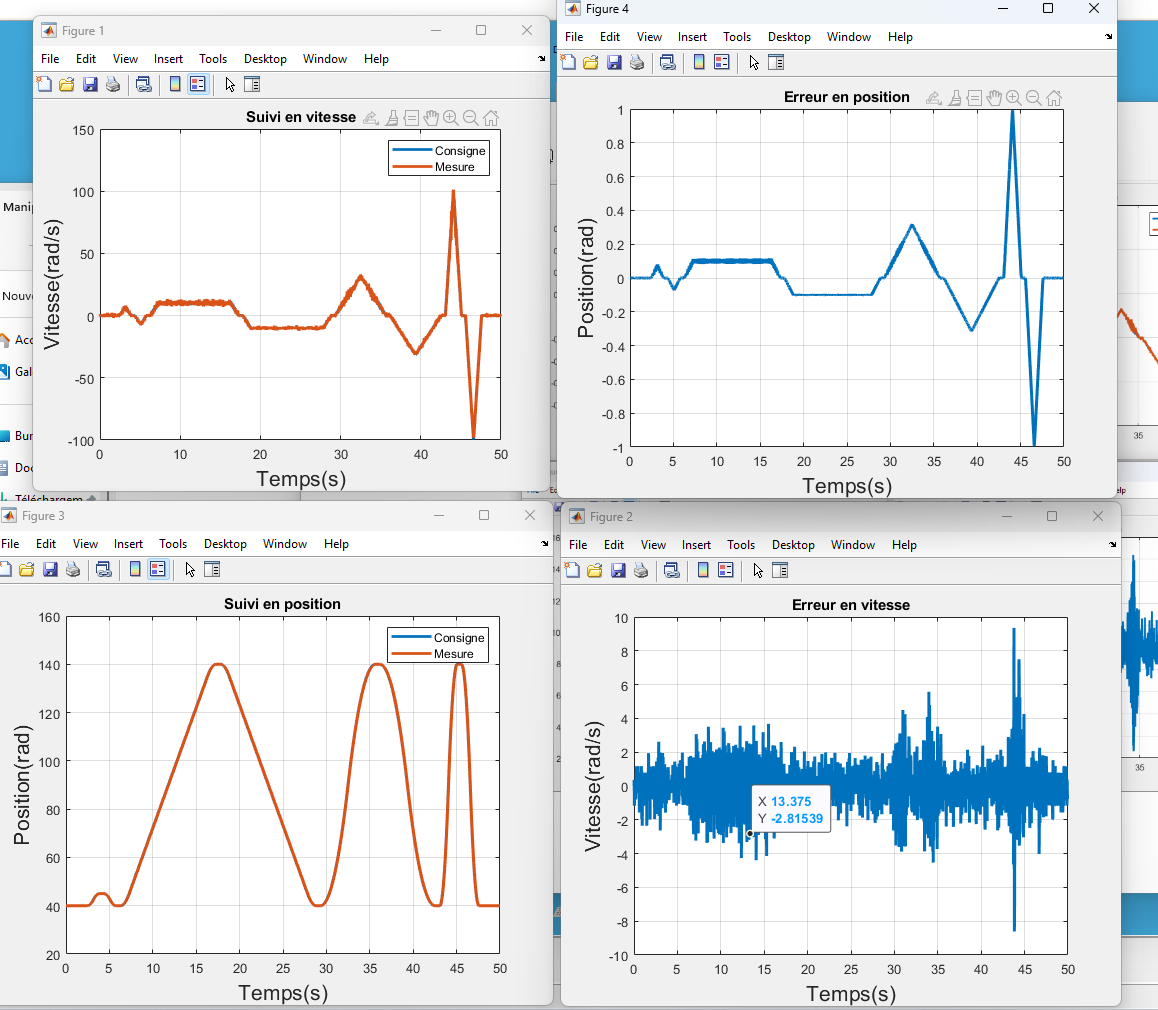
\includegraphics[width=0.72\textwidth]{src/image9.png}
    \caption{Relevés de la Manipulation 3 ($K_p = 100$, $J = J_{\text{charge}}$, Feedforward Off)}
    \label{fig:manip3}
\end{figure}

\textbf{Analyse :}
La prise en compte de la constante d'inertie affine le modèle interne du variateur :
\begin{itemize}
    \item Les bruits à haute fréquence affectant la vitesse et le profil d'erreur de position sont significativement filtrés ;
    \item L'erreur en vitesse est amoindrie lors des deux premières rampes de montée ;
    \item En revanche, au cours de la troisième montée qui impose l'accélération la plus abrupte, l'erreur de traînage augmente temporairement. Ce résultat est cohérent : l'effort inertiel requis ($J \, \frac{\mathrm{d}\Omega}{\mathrm{dt}}$) étant plus important, un système sans anticipation ne peut générer ce surcroît de couple qu'au travers d'une augmentation momentanée de l'écart mesuré.
\end{itemize}

\clearpage

\subsection{Manipulation 4 : \texorpdfstring{$K_p = 100$}{Kp = 100}, Inertie \texorpdfstring{$= 0$}{= 0}, Feedforward On}

Dans cet essai, l'inertie déclarée est réinitialisée à zéro, mais l'anticipation de consigne (\textit{Feedforward}) est activée.

\begin{figure}[H]
    \centering
    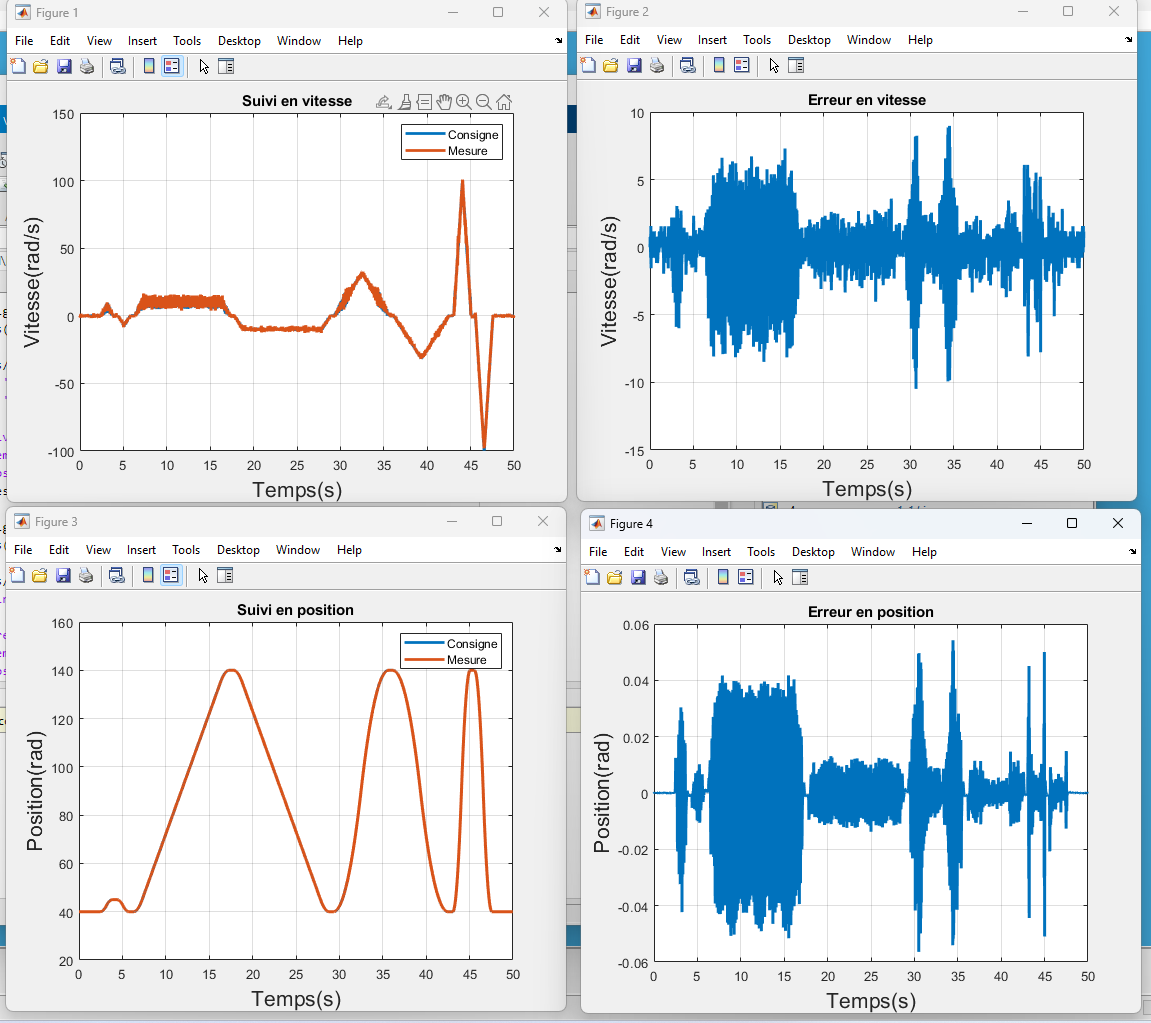
\includegraphics[width=0.72\textwidth]{src/image10.png}
    \caption{Relevés de la Manipulation 4 ($K_p = 100$, $J = 0$, Feedforward On)}
    \label{fig:manip4}
\end{figure}

\textbf{Analyse :}
La confrontation directe avec la manipulation 2 révèle l'efficacité remarquable du \textit{Feedforward} :
\begin{itemize}
    \item L'erreur de poursuite en position devient \textbf{sensiblement nulle sur l'intégralité du cycle}, aussi bien lors des régimes permanents qu'au cours des transitoires d'accélération et de freinage ;
    \item En calculant à chaque pas d'échantillonnage la tension ou le couple requis à partir des dérivées de la consigne (vitesse et accélération souhaitées), le feedforward applique l'effort dynamique de manière prédictive, évitant le décalage temporel inhérent aux boucles de contre-réaction pures.
\end{itemize}

\clearpage

\subsection{Manipulation 5 : \texorpdfstring{$K_p = 100$}{Kp = 100}, Inertie \texorpdfstring{$= J_{\text{charge}}$}{= Jcharge}, Feedforward On}

La dernière manipulation combine tous les réglages optimisés : gain de position élevé ($K_p = 100$), prise en compte de l'inertie ($J = J_{\text{charge}}$) et action anticipatrice (\textit{Feedforward} actif).

\begin{figure}[H]
    \centering
    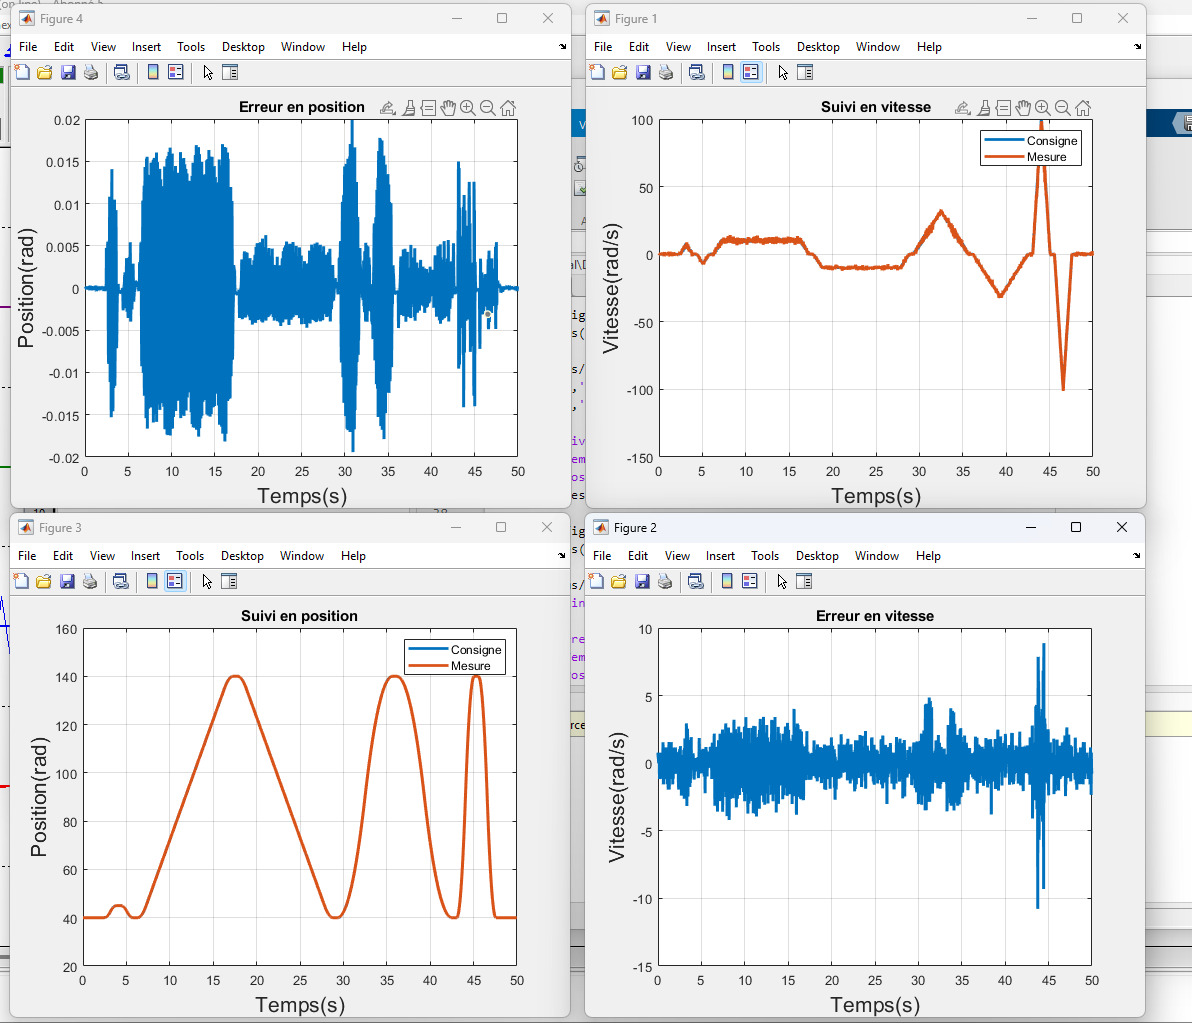
\includegraphics[width=0.72\textwidth]{src/image11.png}
    \caption{Relevés de la Manipulation 5 ($K_p = 100$, $J = J_{\text{charge}}$, Feedforward On)}
    \label{fig:manip5}
\end{figure}

\textbf{Analyse :}
Cette configuration réalise la synthèse optimale :
\begin{itemize}
    \item Les erreurs dynamiques en position et en vitesse atteignent les plus faibles amplitudes mesurées lors de toute la campagne ;
    \item Le système présente une excellente robustesse face aux variations d'accélération, sans dépassement ni vibration résiduelle.
\end{itemize}

\clearpage

\section{Synthèse et interprétation physique des résultats}
\label{sec:synthese_pme}

L'ensemble des expérimentations menées sous PME permet de formaliser les rôles respectifs des organes de correction sur un axe vertical :
\begin{enumerate}
    \item \textbf{Transition frottement sec / frottement visqueux :} À très basse vitesse, l'axe évolue dans le cône d'adhérence mécanique. Un régulateur sous-dimensionné génère une réponse oscillante instable (phénomène de \textit{stick-slip}). Dès que la cinématique franchit le seuil de glissement, le frottement visqueux prend le relais et rétablit un régime continu.
    \item \textbf{Action proportionnelle ($K_p$) :} L'augmentation du gain raidit la commande en boucle fermée, réduisant l'erreur de traînage et forçant le dépassement quasi instantané du seuil de frottement statique sans saccade.
    \item \textbf{Compensation d'inertie ($J$) :} La connaissance de la matrice inertielle affine l'actionneur en adaptant le calibrage de la boucle de couple aux besoins d'accélération ($C_{\text{dyn}} = J \, \dot{\Omega}$).
    \item \textbf{Commande prédictive (\textit{Feedforward}) :} L'anticipation constitue la solution la plus performante pour éliminer le traînage géométrique en boucle fermée, en injectant en boucle ouverte l'effort théorique induit par le profil de mouvement consigne.
\end{enumerate}

\clearpage

% ==============================================================================
% PARTIE II : PROCÉDURE DE RÉGLAGE ORIENTÉ MÉCANIQUE
% ==============================================================================
\part{Procédure de réglage orienté mécanique}

\section{Modélisation mécanique et protocole d'identification}

Le comportement dynamique d'un axe vertical entraîné par un servomoteur synchrone s'exprime au niveau de l'arbre rotorique par le principe fondamental de la dynamique :
\begin{equation}
C_m(t) = J_{\text{tot}} \, \frac{\mathrm{d}\Omega(t)}{\mathrm{dt}} + C_{\text{frott}}(\Omega) + C_{\text{grav}}
\label{eq:modele_dynamique}
\end{equation}
dans lequel :
\begin{itemize}
    \item $C_m(t)$ est le couple électromagnétique utile fourni par le servomoteur ($\text{N}\cdot\text{m}$) ;
    \item $J_{\text{tot}}$ est le moment d'inertie total équivalent ramené à l'arbre moteur ($\text{kg}\cdot\text{m}^2$) ;
    \item $C_{\text{grav}}$ est le couple résistant constant exercé par la charge gravitaire suspendue ($\text{N}\cdot\text{m}$) ;
    \item $C_{\text{frott}}(\Omega) = f_s \, \mathrm{sgn}(\Omega) + f \, \Omega$ caractérise la dissipation par frottement, associant le frottement sec de Coulomb ($f_s$) et le frottement visqueux ($f$).
\end{itemize}

La démarche d'identification préconisée se déroule en trois étapes méthodiques :
\begin{enumerate}
    \item Relevé des couples stabilisés à vitesse constante ($\frac{\mathrm{d}\Omega}{\mathrm{dt}} = 0$) pour isoler $C_{\text{grav}}$ et les coefficients de frottement $f_s$ et $f$ ;
    \item Isolement du couple d'accélération $C_a(t)$ lors d'échelons d'accélération connus pour déterminer l'inertie globale $J_{\text{tot}}$ ;
    \item Calcul des correcteurs de boucle selon les abaques constructeur et validation expérimentale sous fortes sollicitations.
\end{enumerate}

\clearpage

\section{Identification du couple de gravité et des frottements}

\subsection{Relevé des paliers de couple à vitesse stabilisée}

Le banc d'essai est asservi à des consignes de vitesse stabilisées positives (montée) puis négatives (descente) : $\Omega \in \{\pm 25, \pm 50, \pm 75, \pm 100\}\,\text{rad/s}$. En régime établi, l'accélération est nulle ($\dot{\Omega} = 0$), et le couple mesuré se stabilise sur des paliers horizontaux. La figure~\ref{fig:paliers_100} illustre l'acquisition obtenue sous MATLAB pour la vitesse de consigne de $\pm 100\,\text{rad/s}$.

\begin{figure}[H]
    \centering
    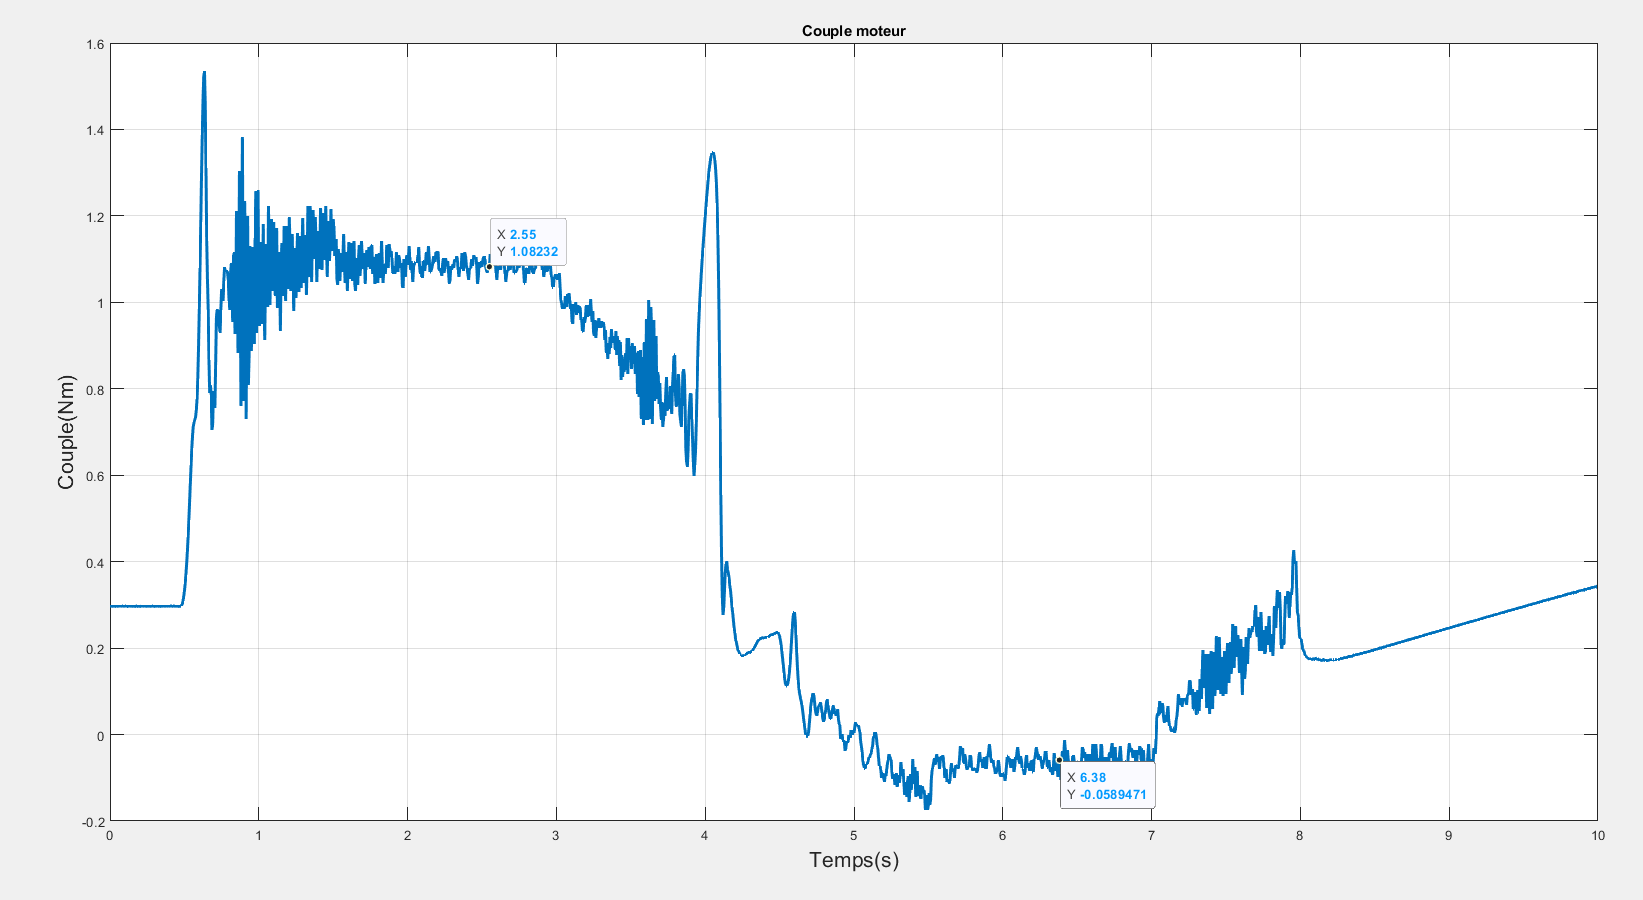
\includegraphics[width=0.72\textwidth]{src/image12.png}
    \caption{Relevé des paliers de couple moteur en régime permanent pour $\Omega = \pm 100\,\text{rad/s}$}
    \label{fig:paliers_100}
\end{figure}

Les valeurs moyennes des paliers de couple mesurées pour l'ensemble des vitesses d'essai sont récapitulées dans le tableau~\ref{tab:paliers}.

\begin{table}[H]
\centering
\begin{tabular}{ccc}
\toprule
\textbf{Vitesse de consigne $\Omega$ (rad/s)} & \textbf{Couple mesuré $C_m$ (N$\cdot$m)} & \textbf{$C_m - C_{\text{grav}}$ (N$\cdot$m)} \\
\midrule
$+100$ & $+1{,}080$ & $+0{,}5721$ \\
$-100$ & $-0{,}075$ & $-0{,}5829$ \\
$+75$  & $+0{,}980$ & $+0{,}4721$ \\
$-75$  & $+0{,}019$ & $-0{,}4889$ \\
$+50$  & $+0{,}940$ & $+0{,}4321$ \\
$-50$  & $+0{,}070$ & $-0{,}4379$ \\
$+25$  & $+0{,}880$ & $+0{,}3721$ \\
$-25$  & $+0{,}140$ & $-0{,}3679$ \\
\bottomrule
\end{tabular}
\caption{Relevé des paliers de couple en fonction de la vitesse de consigne}
\label{tab:paliers}
\end{table}

\subsection{Détermination du couple de gravité \texorpdfstring{$C_{\text{grav}}$}{Cgrav}}

En régime permanent, le modèle dynamique se réduit à :
\begin{equation}
C_m(\Omega) = C_{\text{grav}} + f_s \, \mathrm{sgn}(\Omega) + f \, \Omega
\label{eq:couple_stat}
\end{equation}

Lors de la montée ($\Omega > 0$), le moteur développe :
\begin{equation}
C_{\text{montée}} = C_{\text{grav}} + f_s + f \, \Omega
\end{equation}
Tandis qu'en descente ($\Omega < 0$), l'effort requis devient :
\begin{equation}
C_{\text{descente}} = C_{\text{grav}} - f_s - f \, |\Omega|
\end{equation}

En traçant la caractéristique $C_m = f(\Omega)$ (figure~\ref{fig:courbe_cgrav}), le couple de pesanteur $C_{\text{grav}}$ apparaît comme le décalage vertical moyen de la caractéristique par rapport à l'origine symétrique :
\begin{equation}
C_{\text{grav}} = 0{,}5079\,\text{N}\cdot\text{m}
\end{equation}

Ce couple permanent de $0{,}5079\,\text{N}\cdot\text{m}$ correspond au couple que le moteur doit maintenir à vitesse nulle pour empêcher la chute du chariot mobile sous l'effet de sa propre masse.

\begin{figure}[H]
    \centering
    \begin{minipage}{0.48\textwidth}
        \centering
        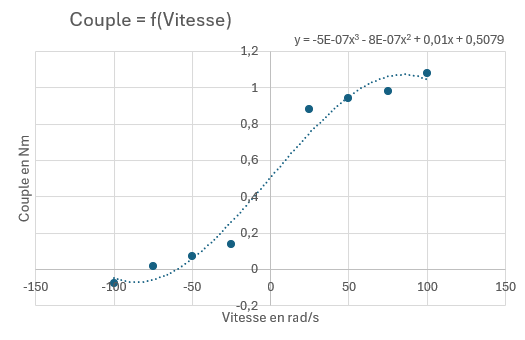
\includegraphics[width=\linewidth]{src/image14.png}
        \caption{Couple mesuré $C_m$ en fonction de la vitesse $\Omega$}
        \label{fig:courbe_cgrav}
    \end{minipage}
    \hfill
    \begin{minipage}{0.48\textwidth}
        \centering
        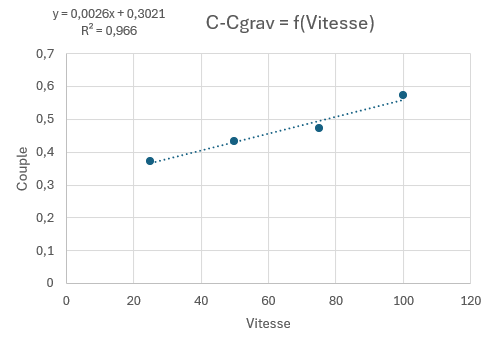
\includegraphics[width=\linewidth]{src/image15.png}
        \caption{Caractéristique de frottement $C_m - C_{\text{grav}} = f(\Omega)$}
        \label{fig:courbe_frott}
    \end{minipage}
\end{figure}

\subsection{Identification des coefficients de frottement visqueux et sec}

Après soustraction du terme de gravité, la composante de frottement pur s'exprime selon :
\begin{equation}
C_m - C_{\text{grav}} = f \cdot \Omega + f_s \, \mathrm{sgn}(\Omega)
\end{equation}

Pour les vitesses positives (figure~\ref{fig:courbe_frott}), la régression linéaire sur les points expérimentaux fournit l'équation de la droite d'ajustement :
\begin{equation}
y = 0{,}0026 \, x + 0{,}3021 \quad \text{avec un coefficient de corrélation} \quad R^2 = 0{,}966
\end{equation}

Par identification directe terme à terme avec $y = f \, \Omega + f_s$, on en déduit avec précision les paramètres mécaniques :
\begin{itemize}
    \item \textbf{Coefficient de frottement visqueux :} $f = 0{,}0026\,\text{N}\cdot\text{m}\cdot\text{s/rad}$ ;
    \item \textbf{Couple de frottement sec (Coulomb) :} $f_s = 0{,}3021\,\text{N}\cdot\text{m}$.
\end{itemize}

\clearpage

\section{Identification du moment d'inertie total équivalent}

Les composantes statiques ($C_{\text{grav}}$, $f_s$, $f$) étant désormais quantifiées, il est possible d'isoler le couple purement dynamique d'accélération $C_a(t)$ sur l'enregistrement temporel en appliquant sous MATLAB l'instruction de compensation :
\begin{equation}
C_a(t) = C_m(t) - f \cdot \Omega(t) - f_s \cdot \mathrm{sgn}(\Omega(t)) - C_{\text{grav}}
\end{equation}

Le signal résultant est représenté sur la figure~\ref{fig:couple_accel}.

\begin{figure}[H]
    \centering
    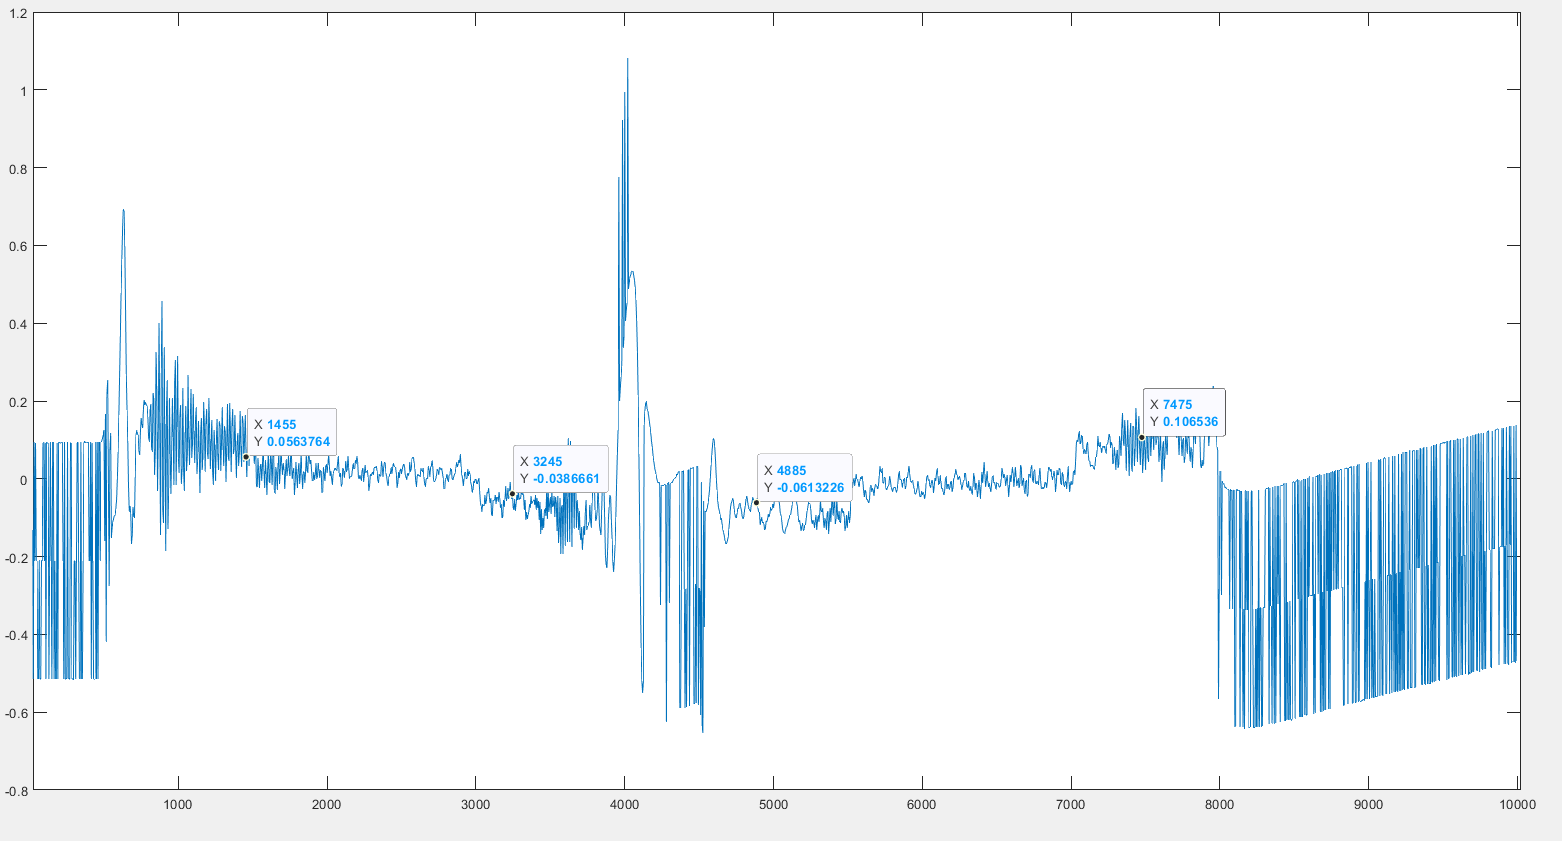
\includegraphics[width=0.72\textwidth]{src/image16.png}
    \caption{Évolution temporelle du couple d'accélération compensé $C_a(t)$}
    \label{fig:couple_accel}
\end{figure}

Le graphe fait distinctement apparaître quatre paliers dynamiques correspondant aux phases d'accélération du cycle d'essai. Par lecture graphique sur ces plateaux stabilisés, la valeur moyenne du couple d'accélération s'établit à :
\begin{equation}
C_a \approx 0{,}10\,\text{N}\cdot\text{m}
\end{equation}

La rampe d'essai imposant une accélération angulaire de $\frac{\mathrm{d}\Omega}{\mathrm{dt}} = 100\,\text{rad/s}^2$, le moment d'inertie total équivalent ramené à l'arbre moteur est donné par :
\begin{equation}
J_{\text{tot}} = \frac{C_a}{\mathrm{d}\Omega/\mathrm{dt}} = \frac{0{,}10}{100} = 0{,}001\,\text{kg}\cdot\text{m}^2 = 1{,}003 \times 10^{-3}\,\text{kg}\cdot\text{m}^2
\label{eq:jtot}
\end{equation}

\clearpage

\section{Synthèse et réglage des correcteurs}

\subsection{Décomposition inertielle de la chaîne cinématique}

L'interface de configuration du variateur sous PME renseigne les moments d'inertie intrinsèques de la partie motorisation (figure~\ref{fig:config_inertie}) :
\begin{itemize}
    \item Inertie propre du rotor moteur : $J_{\text{moteur}} = 0{,}000290\,\text{kg}\cdot\text{m}^2$ ;
    \item Inertie propre du disque de frein : $J_{\text{frein}} = 0{,}000018\,\text{kg}\cdot\text{m}^2$.
\end{itemize}

\begin{figure}[H]
    \centering
    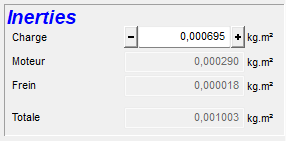
\includegraphics[width=0.42\textwidth]{src/image17.png}
    \caption{Extraction des paramètres inertiels matériels sous l'interface PME}
    \label{fig:config_inertie}
\end{figure}

En retranchant ces composantes internes à l'inertie totale identifiée $J_{\text{tot}}$, on déduit le moment d'inertie effectif de la chaîne cinématique externe ramenée au moteur :
\begin{equation}
J = J_{\text{tot}} - J_{\text{moteur}} - J_{\text{frein}} = 0{,}001003 - 0{,}000290 - 0{,}000018 = 0{,}000695\,\text{kg}\cdot\text{m}^2
\label{eq:j_reel}
\end{equation}

\textbf{Confrontation avec le modèle théorique initial :}
On relève une différence substantielle entre cette inertie mesurée ($J = 6{,}95 \times 10^{-4}\,\text{kg}\cdot\text{m}^2$) et la valeur théorique du chariot seul calculée en équation~\eqref{eq:calcul_inertie} ($J_{\text{charge}} = 3{,}03 \times 10^{-4}\,\text{kg}\cdot\text{m}^2$).
Cette divergence est tout à fait cohérente d'un point de vue physique : le calcul analytique initial ne prenait en compte que la translation de la masse utile ($M = 10{,}5\,\text{kg}$). La méthode d'identification globale intègre quant à elle l'ensemble des éléments tournants de la chaîne cinématique réelle : les étages d'engrenages du réducteur planétaire, l'inertie propre de la poulie motrice et de la poulie de renvoi, la masse de la courroie crantée ainsi que les frottements d'entraînement des roulements à billes.

\subsection{Calcul et implantation des correcteurs de boucle}

À partir des grandeurs physiques identifiées, les paramètres d'asservissement sont dimensionnés conformément aux règles de synthèse industrielle fournies dans l'annexe du TP :

\begin{enumerate}
    \item \textbf{Gain proportionnel de la boucle de vitesse ($k_v$) :}
    Pour garantir un temps de réponse à $5\,\%$ très performant de $t_{r,5\%} = 10\,\text{ms} = 0{,}01\,\text{s}$ :
    \begin{equation}
    k_v = \frac{3}{t_{r,5\%}} = \frac{3}{0{,}01} = 300\,\text{s}^{-1}
    \end{equation}
    \item \textbf{Fréquence d'arrêt intégrale de la boucle de vitesse ($f_i$) :}
    Calée sur la dynamique naturelle de frottement du système :
    \begin{equation}
    f_i = \frac{f}{J_{\text{tot}}} = \frac{0{,}0026}{0{,}001} = 2{,}6\,\text{Hz}
    \end{equation}
    \item \textbf{Filtre passe-bas de vitesse ($f_c$) :}
    Fréquence de coupure paramétrée à $f_c = 600\,\text{Hz}$ pour atténuer les bruits de quantification du codeur incrémental.
    \item \textbf{Gain proportionnel de la boucle de position ($k_p$) :}
    Pour une vitesse de régime $V_0 = 100\,\text{rad/s}$ associée à une erreur de traînage tolérée $\varepsilon_v = 1\,\text{rad}$ :
    \begin{equation}
    k_p = \frac{V_0}{\varepsilon_v} = \frac{100}{1} = 100\,\text{s}^{-1}
    \end{equation}
    \item \textbf{Inertie de charge programmée :} $J = 0{,}000695\,\text{kg}\cdot\text{m}^2$.
\end{enumerate}

\section{Validation expérimentale et limites physiques du banc}

La configuration calculée est injectée dans le variateur afin d'éprouver le comportement de l'asservissement lors d'un cycle dynamique complet : consigne d'aller-retour d'amplitude $250\,\text{rad}$ à une vitesse de croisière de $100\,\text{rad/s}$. L'enregistrement de cet essai est présenté sur la figure~\ref{fig:derniere_manip}.

\begin{figure}[H]
    \centering
    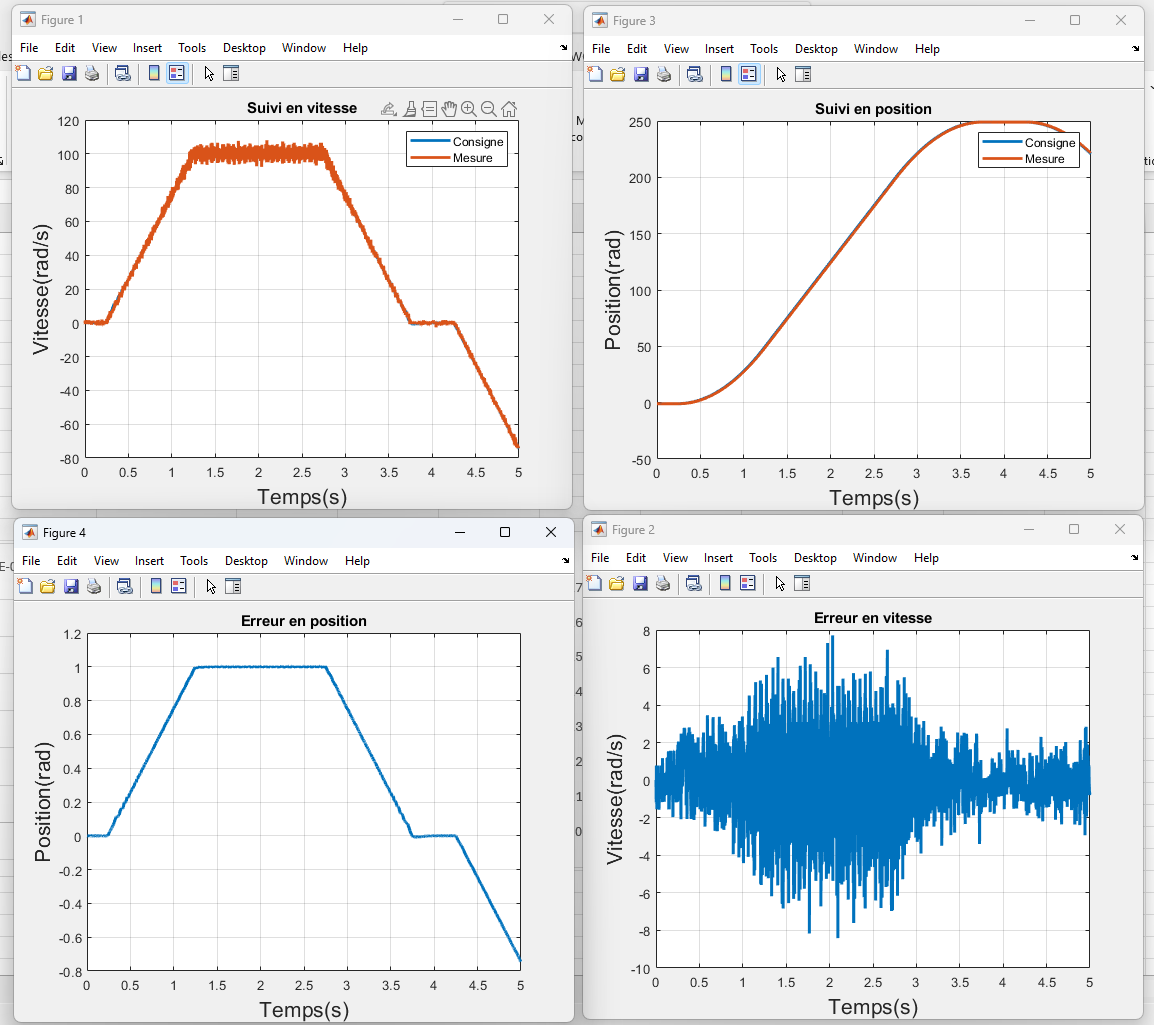
\includegraphics[width=0.72\textwidth]{src/image18.png}
    \caption{Relevé expérimental du cycle aller-retour de $250\,\text{rad}$ à $100\,\text{rad/s}$ (mise en sécurité du variateur)}
    \label{fig:derniere_manip}
\end{figure}

\textbf{Diagnostic de mise en défaut du banc d'essai :}
Au cours de l'exécution de cette consigne exigeante, le variateur décroche brutalement et interrompt le cycle par un déclenchement des sécurités matérielles (« mise en défaut / arrêt machine »). L'analyse physique de cette instabilité met en exergue plusieurs limites critiques :
\begin{itemize}
    \item \textbf{Saturation en couple et limitation en courant :} Le réglage imposé repose sur une bande passante très large ($k_v = 300$, correspondant à un temps de montée de $10\,\text{ms}$). Lors de l'inversion de sens de rotation à pleine vitesse, l'appel de courant commandé excède le seuil de courant de crête admissible par l'onduleur de puissance, déclenchant la protection contre les surintensités.
    \item \textbf{Surpuissance régénérative en descente :} Durant la phase de décélération à la descente, le freinage d'un système vertical cumule la dissipation de l'énergie cinétique et le travail résistant de la gravité. La puissance électrique renvoyée vers le bus continu dépasse les capacités d'absorption du hacheur de freinage, entraînant un défaut de surtension du bus.
    \item \textbf{Enseignements pour le cahier des charges :} Cette expérience démontre les limites intrinsèques d'un dimensionnement linéaire théorique purement fréquentiel lorsqu'il est confronté aux non-linéarités d'actionneurs réels (butées de tension, saturations de courant, dissipation thermique). En milieu industriel, il conviendrait soit d'assouplir le temps de réponse visé ($t_{r,5\%} \approx 25\text{--}35\,\text{ms}$), soit d'adopter un générateur de trajectoire à profil trapézoïdal ou en courbes en $S$ avec limitation stricte de l'accélération et de l'à-coup (\textit{jerk}).
\end{itemize}

\clearpage

% ==============================================================================
% CONCLUSION GÉNÉRALE
% ==============================================================================
\section*{Conclusion générale}
\addcontentsline{toc}{section}{Conclusion générale}

Ce travail pratique a permis d'explorer de manière exhaustive la problématique de l'asservissement en position et en vitesse d'un axe vertical de translation, en comparant les fonctionnalités d'auto-réglage d'un variateur industriel à une démarche rigoureuse d'identification physique.

La première partie consacrée à la commande sous l'environnement PME a mis en évidence :
\begin{itemize}
    \item L'impact délétère des frottements statiques à basse vitesse, provoquant un régime saccadé d'adhérence-glissement (\textit{stick-slip}) sous faible gain proportionnel ;
    \item La nette dissymétrie mécanique entre la montée et la descente générée par la force constante de gravité ;
    \item L'efficacité de l'augmentation du gain $K_p$ pour supprimer le \textit{stick-slip}, ainsi que la supériorité de l'anticipation (\textit{Feedforward}), qui parvient à annuler quasi intégralement les erreurs de traînage dynamique sans altérer la stabilité.
\end{itemize}

La seconde partie a validé expérimentalement une méthode complète d'identification orientée mécanique :
\begin{itemize}
    \item La séparation méthodique des grandeurs a permis d'isoler le couple de gravité ($C_{\text{grav}} = 0{,}5079\,\text{N}\cdot\text{m}$), le couple de frottement sec ($f_s = 0{,}3021\,\text{N}\cdot\text{m}$) et le coefficient de frottement visqueux ($f = 0{,}0026\,\text{N}\cdot\text{m}\cdot\text{s/rad}$) ;
    \item L'identification de l'inertie totale équivalente ($J_{\text{tot}} \approx 0{,}001003\,\text{kg}\cdot\text{m}^2$) a démontré que l'inertie de la chaîne cinématique externe ($J = 6{,}95 \times 10^{-4}\,\text{kg}\cdot\text{m}^2$) est plus de deux fois supérieure à l'inertie du chariot seul, soulignant l'importance des organes de transmission (réducteur, poulies, courroie) trop souvent négligés dans les calculs préliminaires ;
    \item Enfin, l'essai sous forte dynamique a rappelé l'impérieuse nécessité d'intégrer les saturations de l'actionneur (courant maximal, surtension au freinage) dans le gabarit d'asservissement, illustrant le compromis inéluctable entre rapidité en boucle fermée et robustesse matérielle.
\end{itemize}

\clearpage

% ==============================================================================
% TABLES DES ILLUSTRATIONS ET TABLEAUX
% ==============================================================================
\addcontentsline{toc}{section}{\listfigurename}
\listoffigures

\vspace{1cm}

\addcontentsline{toc}{section}{\listtablename}
\listoftables

\end{document}
